\section{Computing scores in a complete search system}
In the previous Chapter we developed the theory underlying term weighting in documents for the purposes of scoring, leading up to vector space models and the basic cosine scoring algorithm. In this Chapter we begin in Section \ref{8.1} with heuristics for speeding up this computation; many of these heuristics achieve their speed at the risk of not finding quite the top K documents matching the query. Some of these heuristics generalize beyond cosine scoring. With Section \ref{8.1} in place, we have essentially all the components needed for a complete search engine. We therefore take a step back from cosine scoring, to the more general problem of computing scores in a search engine. In Section \ref{8.2} we outline a complete search engine, including indexes and structures to support not only cosine scoring but also more general ranking factors such as query term proximity. 

\subsection{Efficient scoring and ranking}\label{8.1}
Before analyzing an efficient version of the cosine ranking algorithm, we focus on the difference between two possible query evaluation techniques: \textbf{TAAT}, or \textbf{term at a time} and \textbf{DAAT}, or \textbf{document at a time}. 

In the \textit{TAAT} technique, the scores for all the documents are computed concurrently, one query term at a time, whereas in the \textit{DAAT} technique we compute the total score for each doc, considering all the query terms, before proceeding to the following one. In general, \textit{TAAT} requires a larger number of documents to be scored, and thus \textbf{more memory} to accumuate their scores before sorting. On the other hand, \textit{DAAT} technique requires \textbf{less memory}, as less documents scores are stored overall. For example, the algorithm in Picture \ref{cosine score} implements a \textit{TAAT} strategy.

In this case we are solving the following problem: find the $k$ documents in the collection "nearest" to the query, i.e. retrieve the top-$k$ largest query-doc cosines. A cosine ranking is defined \textbf{efficient} if the cosine values are computed efficiently and if the $k$ largest cosines are chosen efficiently. Since we're dealing with sparse query/documents vector, the problem of finding the $k$-nearest neighbors to a query vector is a solvable problem (more difficult for high-dimensional spaces and dense vectors).

\subsubsection{TAAT}
In this case the idea for an efficient ranking is to pick the $k$-nearest neighbors without totally ordering all the scores. In other words, let $J$ be the number of docs with non-zero cosines, our goal is to retrieve the $k$ best of these $J$ scores, rather that $N$.

An alternative is to use a MaxHeap to select the top-$k$. A MaxHeap is a priority queue with the following properties:

\begin{itemize}
    \item it is a complete binary tree, i.e. if a node is stored at index $k$, then its left/right children are stored at index $2k + 1$ and $2k + 2$;
    \item node's values are $\geq$ than the values of the children.
\end{itemize}

Given a complete array of \textit{accumulators}, $2J$ comparisons are required to build a MaxHeap; then, each of the $k$ "winners" is retrieved in $\log J$ steps. Thus, the total cost is $2J + k\log J$.

Once we established a method for fast ranking, we now focus on some strategies for fast scoring. The main idea is to assume that each query term occurs only once, i.e. $tf = 1$: in this way, each query term has not any weight, so in the ranking phase the query vector is not needed to be normalized. In this sense, $idf$ is only used for computing $wf_{t,d}$ and not for $wf_{t,q}$. The motivations for this choice relies on the following inequality, where $\Vec{q}$ represents the normalized vector of the query $q$, while $\Vec{Q}$ is the un-normalized one, i.e. all the nonzero components are equal to 1:

$$
\Vec{Q} \cdot \Vec{d_1} >  \Vec{Q} \cdot \Vec{d_2} \Longleftrightarrow \Vec{q} \cdot \Vec{d_1} >  \Vec{q} \cdot \Vec{d_2}
$$

These simplifications lead to the algorithm in Picture \ref{fast cosine score}.

\begin{figure}[h!]
		\centering
		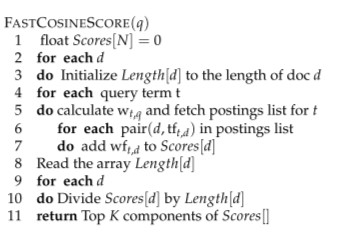
\includegraphics[scale = 2.0]{img/fast cosine score.jpg}
		\label{fast cosine score}
        \caption{A faster algorithm for computing vector space scores}
\end{figure}

Some notes:

\begin{itemize}
    \item Line 7: since $wf_{t,q} = 1$, the multiply-add of algorithm \ref{cosine score} becomes an addition here;
    \item Line 11: the top-$k$ documents are retrieved using the MaxHeap strategy described above.
\end{itemize}

\subsubsection{DAAT}
In this case the idea is to use a binary MinHeap of $k$ elements. It takes $O(\log k)$ operations to insert a new \textit{accumulator}, then $k$ winners are read off in order. In this sense, the goal is to keep the top-$k$ documents seen so far, by using a binary MinHeap and performing the following operations when processing a new document $d'$ with score $s'$:

\begin{enumerate}
    \item Get the current minimum $h_m$ of heap (cost is $O(1)$);
    \item If $s' < h_m$, skip to the next document;
    \item if $s' \geq h_m$, perform an heap deletion of the root (cost is $O(\log k)$), and add $s':d'$ (cost is $O(\log k)$)
\end{enumerate}

Clearly, in the worst case scenario we have to add to the min heap all the new documents. An example of the functioning of this approach is given in Picture \ref{min heap ex}: as we can see, documents 6, 10 and 11 are not added to the MinHeap.

\begin{figure}[h!]
		\centering
		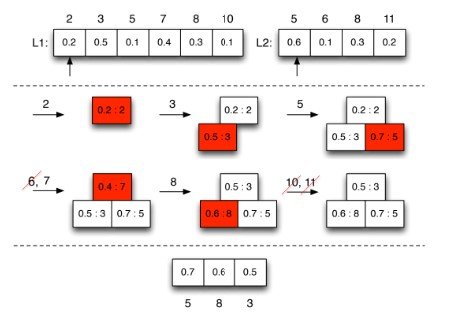
\includegraphics[scale = 2.0]{img/min heap ex.jpg}
		\label{min heap ex}
        \caption{Example of MinHeap of 3 elements}
\end{figure}

\subsubsection{WAND}

Another possible method for query evaluation in the \textit{DAAT} approach is provided by the \textbf{WAND scoring}. Notice that the normal DAAT still computes all the $J$ scores (i.e. all the non-zero scores), while the WAND approach is the following:

\begin{itemize}
    \item we maintain a running threshold score, e.g. the $k$-th highest score computed so far, which corresponds to the least score in the MinHeap;
    \item we prune away all the docs whose cosine scores are guaranteed to be below the current threshold;
    \item we compute the exact cosine scores for only the un-pruned documents, that are much less than the original $J$ scores.
\end{itemize}

In this sense, the WAND scoring technique is based on a two-level evaluation:

\begin{enumerate}
    \item The first level evaluation is used to quickly establish whether a document merits to be fully evaluated, i.e. whether it has a chance of being a top-$k$ document. Notice that this phase cannot lead to \textit{false negatives}, i.e. all the potential matches have to be kept, while on the other hand it could lead to few \textit{false positives};
    \item The second level consists on the full evaluation of the candidates retrieved in the first phase to enter the MinHeap.
\end{enumerate}

In this approach the \textbf{postings are ordered} by docID, and we assume there exists a \textbf{special iterator} on the postings with the following form: "go to the first docID $\geq$ X", i.e. an iterator that can skip blocks of documents. In a typical state, we have a \textbf{"finger"} at some docID in the postings of each query term, and each finger only moves to the right, i.e. to larger docIDs, by using the special iterator if needed. Clearly, the invariant is that all the docIDs lower than any finger have already been processed, meaning that either these docIDs have been pruned away or their cosine scores have been computed (in this case we can have either true positives or false positives).

Moreover, we assume that each query term $t$ is associated with an \textbf{upper bound} $UB_t$ on its maximal contribution to any document score in the postings list:

$$
UB_t \geq \alpha_t \text{max}(w(t,d_1), w(t,d_2), ..)
$$
, where $w(t,d_i)$ is the weight of a term, given by \textit{tf-idf}.

In addition, we set a \textbf{threshold} $\tau$, which defines the min score of the MinHeap, and whenever a documents $d$ succeeds in entering the MinHeap, the threshold grows.

A crucial operation in WAND is the \textbf{pivoting}, i.e. the searching of the \textbf{pivot} element: the pivot element is the first term for which $\sum_t UB_t > \tau$. If we have a situation like the one of Picture \ref{pivot}, the pivot is represented by the term \textit{in}.

\begin{figure}[h!]
		\centering
		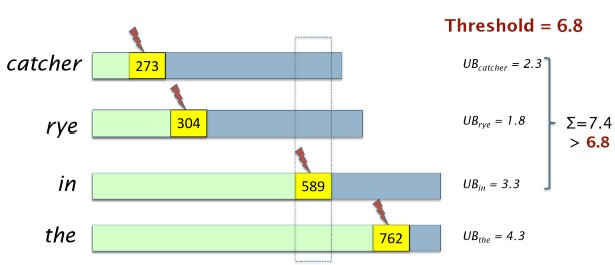
\includegraphics[scale = 1.5]{img/pivot example.jpg}
		\label{pivot}
        \caption{Pivot}
\end{figure}

Once the pivot is determined, all the fingers are moved to the position of the pivot, using the iterator we introduced before: in this way, we perform the pruning operation of the documents that have no hope of being in the top-$k$.

\begin{figure}[h!]
		\centering
		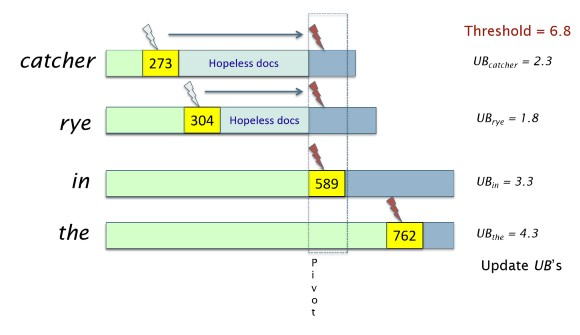
\includegraphics[scale = 1.5]{img/wand pruning.jpg}
		\label{pruning}
        \caption{Pruning phase}
\end{figure}

Finally, if the docID of the pivot is present in all the three postings, we compute its full cosine score, otherwise we move the fingers and we consider another pivot.

The results of the WAND algorithm show that it leads to a 90+\% reduction in the score computation, and that it provides the best gains on longer queries. Notice that the functioning of the algorithm is not specific for the cosine ranking, but we only need the scoring metric to be additive by term. Finally, we notice that TAAT, DAAT, WAND and other variants of this algorithm provide a \textbf{safe ranking}, i.e. we're guaranteed that the top-$k$ documents are associated with the $k$ highest scored documents.

\subsubsection{Block-Max}
\textbf{Block-Max} represents a variant of the WAND algorithm. While in WAND algorithm the maximum "impact score" for each term/postings list is stored, the Block-Max algorithm stores the maximum "impact score" for each \textbf{block} of a compressed inverted list in uncompressed form. This behaviour enables the skip of large parts of the lists, without decompressing, so it speedups WAND. In particular, the algorithm splits the inverted lists into blocks of 64 or 128 docIDs, s.t. each block can be uncompressed separately; moreover, for each compressed block an additional table is created, which stores for each block:

\begin{itemize}
    \item the maximum (or minimum) docID;
    \item the maximum impact value for each block;
    \item the block size.
\end{itemize}

As in WAND, the \textbf{special iterator} is implemented to avoid decompressing blocks that are not relevant.

From Picture \ref{block max} we notice that for each block we maintain an upper bound approximation of the impact scores of each list, which corresponds to the maximum of the values, as we said before. Moreover, inside each block there may be many 0 values, that can be retrieved by decompressing the block. Finally, we notice that the blocks are not uniform in size.

\begin{figure}[h!]
		\centering
		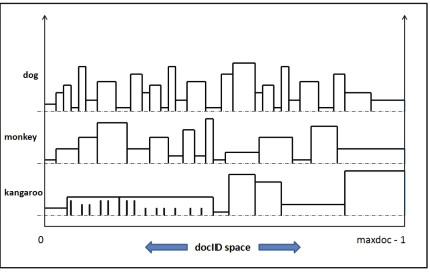
\includegraphics[scale = 1.5]{img/block max.jpg}
		\label{block max}
        \caption{Blocks in Block Max algorithm}
\end{figure}

The \textit{Block Max} algorithm is implemented as follows:

\begin{enumerate}
    \item Sort the list from top to bottom, according the the docIDs of the current postings in the lists, as in WAND;
    \item Find the pivot ID as in WAND;
    \item Use the \textit{global maximum scores} ($UB_t$) to determine a candidate pivot, as in WAND;
    \item Use the \textit{block maximum scores} (which is $< UB_t$) to check if the candidate pivot is a real pivot.
    \begin{itemize}
        \item If it is a real pivot, move the current pointers of the previous query terms to the first postings in their lists, with docIDs $\geq$ the pivot ID, like in WAND;
        \item Otherwise, move them to ID = min(ID$_i$), where the various ID$_i$ are the maximum docIDs in the current blocks.
    \end{itemize}
\end{enumerate}

Picture \ref{block max res} shows the average query processing time of different algorithms w.r.t. different number of terms in the query, while Picture \ref{block max res 2} show the average number of processed documents by the algorithms. In both cases we notice that Block Max algorithm obtains the best performances.

\begin{figure}[h!]
		\centering
		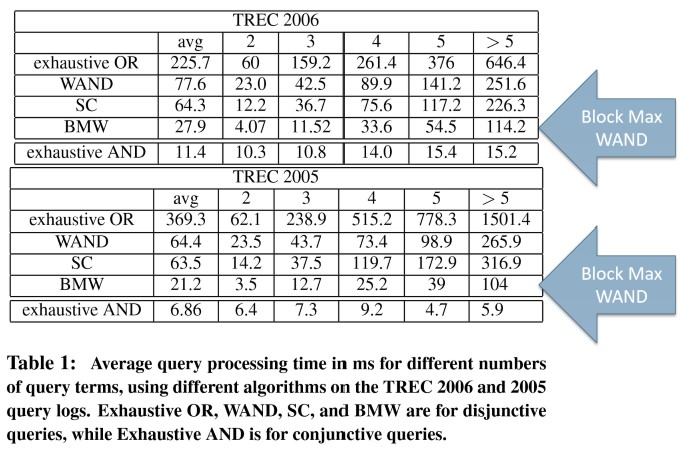
\includegraphics[scale = 1.5]{img/block max results.jpg}
		\label{block max res}
        \caption{Comparison of different retrieval algorithms}
\end{figure}

\begin{figure}[h!]
		\centering
		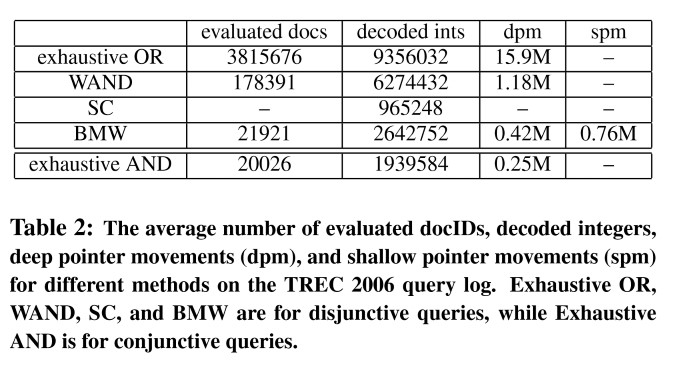
\includegraphics[scale = 1.5]{img/block max results 2.jpg}
		\label{block max res 2}
        \caption{Comparison of different retrieval algorithms}
\end{figure}

\subsubsection{Inexact top-$k$ retrieval}
Thus far, we have focused on retrieving precisely the $k$ highest-scoring documents for a query. We now consider schemes by which we produce $k$ \textbf{documents that are likely to be among the $k$ highest scoring documents} for a query. In doing so, we hope to \textbf{dramatically lower} the \textbf{cost of computing} the $k$ documents we output, without materially altering the user’s perceived relevance of the top $k$ results. Consequently, in most applications it suffices to retrieve $k$ documents whose scores are very close to those of the $k$ best.

In general, the inexact top-$k$ retrieval is not a bad thing from the user's point of view, since the ranking function is only a proxy for the user's happiness, so the corresponding result may not be exact w.r.t. the user's will.

As an example, the WAND algorithm can be made inexact on two possible ways:

\begin{itemize}
    \item the first is a \textbf{safe} aggressive pruning, and it consists of considering smaller values for $k$: in this way, the threshold $\tau$ becomes higher, resulting in more pruning of low-scoring documents;
    \item the second is an \textbf{unsafe} aggressive pruning, and it consists of considering larger values of the threshold $\tau$, for example by considering a new threshold $\tau' = F \cdot \tau$, where $F \geq 1$ being a tunable parameter: in this way, a document deserves to be fully evaluated only if the final score is likely much greater than the current threshold $\tau$.
\end{itemize}

However, we now consider a series of ideas designed to \textbf{eliminate a large number of documents} without computing their cosine scores. The heuristics have the following two-step scheme:

\begin{enumerate}
    \item Find a set $A$ of documents that are contenders, where $k < |A| << N$. $A$ does not necessarily contain the $k$ top-scoring documents for the query, but is likely to have many documents with scores near those of the top $k$;
    \item Return the $k$ top-scoring documents in $A$. 
\end{enumerate}

From the descriptions of these ideas it will be clear that many of them require parameters to be tuned to the collection and application at hand, but it is important to notice that this approach can be used also for other (non-cosine) scoring functions.

\underline{\textbf{\textbf{Index elimination}}}

For a multi-term query $q$, it is clear that we compute the cosine only for the documents containing at least one of the query terms: we can take this observation further considering the following heuristics:

\begin{enumerate}
    \item We only consider documents containing query terms whose $idf$ exceeds a preset threshold, i.e. we only traverse the postings for terms whose $idf$ exceeds the threshold. Using this technique, the set of documents for which we compute cosines is greatly reduced. One way of viewing this heuristic: low $idf$ terms are treated as stop words and do not contribute to scoring. For instance, on the query \textit{catcher in the rye}, we only traverse the postings for \textit{catcher} and \textit{rye};
    \item We only consider documents that contain many (and as a special case, all) of the query terms: a danger of this scheme is that by requiring all (or even many) query terms to be present in a document before considering it for cosine computation, we may end up with fewer than $K$ candidate documents in the output. However, this strategy is quite easy to implement.
\end{enumerate}

\underline{\textbf{\textbf{Champion lists}}}

The idea of \textbf{champion lists} is to \textbf{precompute}, for each term $t$ in the dictionary, the set of the $r$ \textbf{documents} with the \textbf{highest weights} for $t$; the value of $r$ is chosen in advance. For $tf-idf$ weighting, these would be the $r$ documents with the highest $tf$ values for term $t$. We call this set of $r$ documents the \textit{champion list} for term $t$. 

Now, given a query $q$ we create a set $A$ as follows: we take the union of the champion lists for each of the terms comprising $q$. We now restrict cosine computation to only the documents in $A$. 

A critical parameter in this scheme is the \textbf{value $r$}, which is highly \textbf{application dependent}: intuitively, $r$ should be large compared with $k$, but it is set at the time of index construction, whereas $k$ is application dependent and may not be available until the query is received. In general, there is no reason to have the same value of $r$ for all terms in the dictionary; it could for instance be set to be \textbf{higher for rarer terms}.

\underline{\textbf{\textbf{Static quality scores and ordering}}}

We now further develop the idea of champion lists, in the somewhat more general setting of \textit{static quality scores}. In many search engines, we have available a \textbf{measure of quality} $g(d)$ for each document $d$ that is \textbf{query-independent} and thus \textbf{static}, where $0 \leq g(d) \leq 1$. For instance, this quantity may refer to the number of citations of a paper, or the PageRank score etc..

The \textbf{net score} for a document $d$ is some combination of \textbf{quality/authority}, defined by $g(d)$, together with the query-dependent score representing the \textbf{relevance}, for example the cosine score:

$$
\text{net-score}(q,d) = g(d) + \text{cosine}(q,d) = g(d) + \frac{\Vec{q} \cdot \Vec{d}}{|\Vec{q}||\Vec{d}|}
$$

Notice that $g(d)$ and $\text{cosine}(q,d)$ could be weighted in some way.

The \textbf{first idea} is to \textbf{order} the \textbf{documents} in the postings list for each term by \textbf{decreasing value} of $g(d)$. This allows us to perform the postings intersection algorithm of Picture \ref{intersection}, so we can concurrently traverse the query terms' postings for both postings intersection and cosine score computation. This idea is a direct extension of champion lists: for a well-chosen value $r$, we maintain for each term $t$ a global champion list of the $r$ documents with the highest values for $g(d) + tf-idf_{t,d}$. Then, at query time we only compute the net scores for documents in the union of these global champion lists. Intuitively, this has the effect of focusing on documents likely to have large net scores. 

The reason why we perform an ordering by $g(d)$ is that under $g(d)$ ordering top-scoring docs are likely to appear early in postings traversal, so in time-bound applications, for example, this strategy allows us to stop the postings traversal early with good results, since we avoid computing scores for non-relevant documents.

The \textbf{second idea} is to maintain for each term $t$ \textbf{two postings lists} consisting of \textbf{disjoint sets of documents}, each sorted by $g(d)$ values. The first list, which we call \textit{high}, contains the $m$ documents with the highest $tf$ values for $t$. The second list, which we call \textit{low}, contains all other documents containing $t$. When processing a query, we first scan only the \textit{high} lists of the query terms, computing net scores for any document on the \textit{high} lists of all (or more than a certain number of) query terms. If we obtain scores for $k$ documents in the process, we terminate. If not, we continue the scanning into the \textit{low} lists, scoring documents in these postings lists.

More generally, this second idea belongs to a more general aproach that consists of exploiting \textbf{tiered indexes}: the idea of these indexes is to break the postings up into a hierarchy of lists of decreasing importance, where the importance may be defined by $g(d)$ or by $g(d) + tf-idf(t,d)$. The structure of tiered indexes is provided in Picture \ref{tier}.

\begin{figure}[h!]
		\centering
		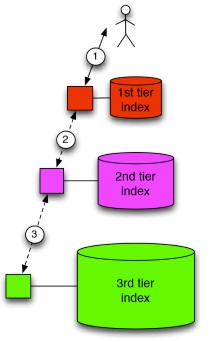
\includegraphics[scale = 1.5]{img/tiered index 2.jpg}
		\label{tier}
        \caption{Structure of a tiered index}
\end{figure}

As we can see:

\begin{itemize}
    \item The tiered index is composed of several sub-indexes;
    \item Former sub-indexes are small and keep more important documents, while later sub-indexes are larger and keep less important documents;
    \item At query time, only the top tier indexes are used to retrieve the top-$k$ documents: if the retrieval fails, it proceeds to lower tiers.
\end{itemize}

This method is characterized by the following issues:

\begin{itemize}
    \item The choice of the value of importance according to which a document is placed in each tier;
    \item How to place documents in different tiers (offline);
    \item At which tier do we stop the query processing (online).
\end{itemize}

\underline{\textbf{\textbf{Impact ordering}}}

Thus far, we've only considered common ordering of documents, either by docID or by static quality score, e.g. net-score. However, this ordering imposes a DAAT scoring, i.e. a concurrent traversal of all of the query terms' postings computing the score for each document as we encounter it. We now consider a TAAT approach, that allows to preclude such a concurrent traversal.

The idea is to order the documents $d$ in the postings list of term $t$ by decreasing order of $tf(t,d)$. Thus, the ordering of documents will vary from one postings list to another, and we cannot compute scores by a concurrent traversal of the postings lists of all query terms. Given postings lists ordered by decreasing order of $tf(t,d)$, two ideas have been found to significantly lower the number of documents for which we accumulate scores: 

\begin{enumerate}
    \item When traversing the postings list for a query term $t$, we stop either after a fixed number of documents $r$ have been seen, or after the value of $tf(t,d)$ has dropped below a threshold. Then, we take the union of the resulting sets of documents, and we compute the scores only for the documents in this union;
    \item When accumulating cosine scores we only consider the query terms in decreasing order of $idf$, so that the query terms likely to contribute the most to the final scores are considered first.
\end{enumerate}

\underline{\textbf{\textbf{Cluster pruning}}}

In cluster pruning we have a preprocessing step during which we \textbf{cluster the document vectors}. Then at query time, we consider only documents in a small number of clusters as candidates for which we compute cosine scores. 

Specifically, the preprocessing step is as follows:

\begin{enumerate}
    \item Pick $\sqrt{N}$ documents at random from the collection, the \textit{leaders}. Alternatively, we can use k-means to choose them;
    \item For each document that is not a \textit{leader} (the \textit{followers}), we pre-compute its nearest \textit{leader}. Intuitively, the expected number of followers for each leader is $\approx N / \sqrt{N} = \sqrt{N}$;
\end{enumerate}

Next, query processing proceeds as follows:

\begin{enumerate}
    \item Given a query $q$, find the \textit{leader} $L$ that is closest to $q$. This entails computing cosine similarities from $q$ to each of the $\sqrt{N}$ \textit{leaders};
    \item The candidate set $A$ consists of $L$ together with its \textit{followers}. We compute the cosine scores for all documents in this candidate set;
\end{enumerate}

A scheme of this approach is provided in Picture \ref{cluster pruning}.

\begin{figure}[h!]
		\centering
		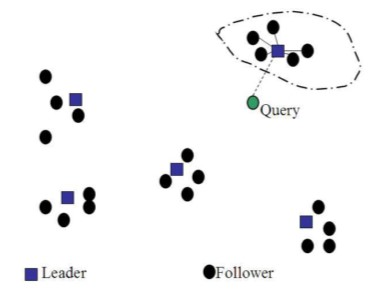
\includegraphics[scale = 1.5]{img/cluster pruning.jpg}
		\label{cluster pruning}
        \caption{Cluster pruning}
\end{figure}

The use of randomly chosen \textit{leaders} for clustering is fast and likely to reflect the distribution of the document vectors in the vector space: a region of the vector space that is dense in documents is likely to produce multiple \textit{leaders} and thus a finer partition into sub-regions. 

Variations of cluster pruning introduce additional parameters $b_1$ and $b_2$, both of which are positive integers. In the pre-processing step we attach each \textit{follower} to its $b_1$ closest leaders, rather than a single closest leader. At query time we consider the $b_2$ leaders closest to the query $q$. Clearly, the basic scheme above corresponds to the case $b_1 = b_2 = 1$. Further, increasing $b_1$ or $b_2$ increases the likelihood of finding $k$ documents that are more likely to be in the set of true top-scoring $k$ documents, at the expense of more computation. In general, this variation implements the concept of \textit{fuzzy/soft clustering}, and in general it produces larger clusters.


\subsection{Components of an IR system}\label{8.2}
In this section we combine the ideas developed so far to describe a rudimentary search system that retrieves and scores documents. We first develop further ideas for scoring, beyond vector spaces. Following this, we will put together all of these elements to outline a complete system.

\subsubsection{Tiered index}
The first component is the \textit{tiered index}, which we already presented in the previous section.

\subsubsection{Query-term proximity}
Especially for \textbf{free text queries} on the web, i.e. a set of terms typed into a query box, users prefer a \textbf{document} in which \textbf{most} or all of the \textbf{query terms appear close to each other}, because this is evidence that the document has text focused on their query intent. 

Consider a query with two or more query terms, $t_1, t_2,.., t_k$. Let $\omega$ be the \textbf{width of the smallest window} in a document $d$ that \textbf{contains all the query terms}, measured in the number of words in the window. For instance, if the document were to simply consist of the sentence "The quality of mercy is not strained", the smallest window for the query "strained mercy" would be 4. Intuitively, the \textbf{smaller} that $\omega$ is, the \textbf{better} that $d$ matches the query. In cases where the document does not contain all of the query terms, we can set ω to be some enormous number. We could also consider variants in which only words that are not stop words are considered in computing $\omega$. Such \textbf{proximity-weighted scoring functions} are a departure from pure cosine similarity and closer to the “soft conjunctive” semantics that Google and other web search engines evidently use.

How can we design such a proximity-weighted scoring function to depend on $\omega$? We treat the integer $\omega$ as yet another \textbf{feature} in the \textbf{scoring function}, whose importance is assigned by \textbf{machine learning}, as will be developed in the following sections.

\subsubsection{Query parsers}
Common search interfaces tend to \textbf{mask query operators} from the end user, in order to hide the complexity of these operators from the largely non-technical audience for such applications, inviting \textbf{free text queries}. Given such interfaces, how should a search equipped with indexes for various retrieval operators treat a query such as "rising interest rates"? 

The answer of course depends on the user \textbf{population}, the \textbf{query distribution} and the \textbf{collection of documents}. Typically, a \textbf{query parser} is used to translate the user-specified keywords into a query with various operators that is executed against the underlying indexes:

\begin{enumerate}
    \item Run the user-generated query string as a \textit{phrase query} "rising interest rates" and rank the matching docs using vector space scoring;
    \item If fewer than $K$ documents contain the phrase "rising interest rates", run the two 2-term phrase queries "rising interest" and "interest rates"; rank these using vector space scoring, as well;
    \item If we still have fewer than ten results, run the vector space query consisting of the three individual query terms
\end{enumerate}

Each of these steps (if invoked) may yield a list of scored documents, for each of which we compute a score. This score must combine contributions from vector space scoring, static quality, proximity weighting and potentially other factors. This demands an \textbf{aggregate scoring function} that accumulates \textit{evidence} of a document’s relevance from multiple sources. How do we devise a query parser and how do we devise the aggregate scoring function? 

The answer depends on the setting. In many enterprise settings we have application builders who make use of a toolkit of available scoring operators, along with a query parsing layer, with which to manually configure the scoring function as well as the query parser. This setting works in collections whose characteristics change infrequently. \textbf{Web search} on the other hand is faced with a \textbf{constantly changing document collection} with new characteristics being introduced all the time. It is also a setting in which the number of scoring factors can run into the hundreds, making hand-tuned scoring a difficult exercise. To address this, it is becoming increasingly common to use \textbf{machine-learned scoring}, that we will explore later in the notes.

\subsubsection{Putting it all together}
The overall search system that supports free-text queries, as well as Boolean, zone and filed queries is represented in Picture \ref{complete system}: note that the paths are shown primarily for a free text query.

\begin{figure}[h!]
		\centering
		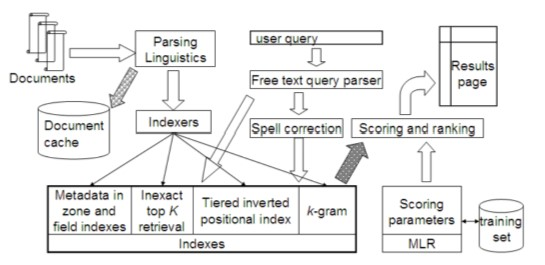
\includegraphics[scale = 1.8]{img/complete system.jpg}
		\label{complete system}
        \caption{A complete search system}
\end{figure}

The steps are the following:

\begin{enumerate}
    \item The documents stream in for \textbf{parsing} and \textbf{linguistic processing} (tokenization, stemming etc..). The resulting stream of tokens feeds into two modules:

    \begin{itemize}
        \item First, we retain a copy of each parsed document in a \textbf{document cache}. This will enable us to generate \textbf{results snippets}, i.e. snippets of text accompanying each document in the results list for a query. This snippet tries to give a succinct explanation to the user of why the document matches the query;
        \item A second copy of the tokens is fed to a bank of \textbf{indexers}. 
    \end{itemize}

    \item The \textbf{indexers} create a bank of indexes including zone and field indexes that store the metadata for each document, tiered indexes, indexes for spelling correction and structures for accelerating inexact top-$k$ retrieval;
    \item A \textbf{free text user query} is sent down to the indexes both directly and through a module for generating spelling-correction candidates;
    \item \textbf{Retrieved documents} are passed to a \textbf{scoring module} that computes scores based on machine-learned ranking (MLR) for \textbf{scoring} and \textbf{ranking} documents;
    \item Finally, these ranked documents are rendered as a \textbf{results page}.
\end{enumerate}

